\subsubsection{Implementacion 1}

\textbf{Explicación Assembler}

La matriz se recorre de manera análoga a las implementaciones anteriores, utilizamos dos ciclos, uno para recorrer las filas y otro las columnas.

Esta implementación utiliza llamados a funciones de C para la transformación de formatos del pixel.

Para realizar ésto, guardamos en cada doubleWord del registro XMM0 los valores pasados como parámetro en la función, que corresponden al dato a sumar a cada componente del pixel.
Además, creamos un vector en donde vamos a guardar el resultado de llamar a la función para transformar un pixel a formato HSL (utilizando una función C ya implementada).

\begin{figure}[ht!]
\centering
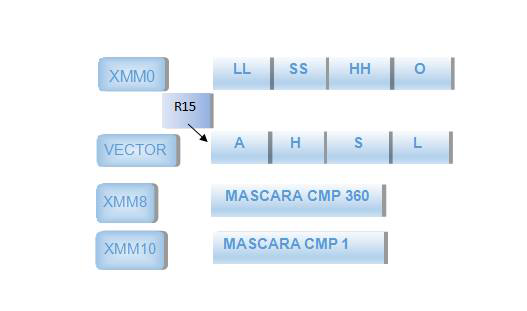
\includegraphics[width=80mm]{imagenes/hsl/hsl1-1.png}
\caption{Desarrollo de HSL-ASM1.}
\end{figure}

Una vez realizado esto, procedemos a realizar las operaciones debidas a los píxeles iterando uno a uno todos los píxeles de la imagen.

En cada iteración comenzamos transformando las componentes del pixel rgb a componentes HSL con la función implementada en C correspondiente, usando el vector creado por nosotros como contenedor del resultado.

\begin{wrapfigure}{r}{70mm}
\centering
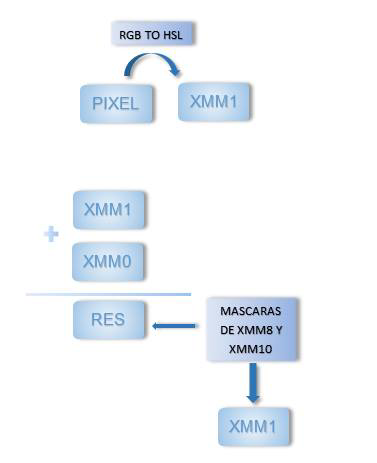
\includegraphics[width=70mm]{imagenes/hsl/hsl1-2.png}
\caption{Desarrollo de HSL-ASM1.}
\end{wrapfigure}

Una vez obtenido este resultado, lo cargamos en el registro XMM1 y le sumamos los datos correspondientes, que previamente habiamos guardado en XMM0. Luego controlamos que los valores obtenidos sean válidos y correctos según las fuciones dadas por la cátedra, implementando las funciones condicionales analizando si se cumplen las condiciones desde el final hacia el principio. Es decir, vemos si el último caso de la función condicional es válido. Si es válido, escribimos ese valor y procedemos a analizar el caso anterior de la función. Si también correcto cambiamos el valor escrito anteriormente por este, quedando como resultado final de la función el primer caso valido de la función.

Una vez finalizadas estas operaciones, guardamos el resultado en nuestro vector y procedemos a volver a convertir las componentes HSL a componentes rgb utilizando la función C correspondiente, la cual guarda el resultado final del pixel en la imagen.

Una vez terminadas todas las iteraciones, liberamos la memoria correspondiente a nuestro vector y terminamos la función.

\newpage

\subsubsection{Implementacion 2}

\textbf{Explicación Assembler}

En esta implementación realizamos el filtro HSL completamente en código assembler.

Para eso, realizamos la misma implementación de suma que la primera implementación del filtro explicada anteriormente.

Para realizar la conversión del formato rgb al formato HSL, transformamos el tamaño cada componente del pixel de byte a doubleword y las guardamos en el registro XMM0, los convertimos a valores en punto flotante y guardamos la componente de transparencia, dado que no se modifica, en el vector.

Calculamos el máximo y el mínimo entre las componentes rgb del pixel y con estos valores procedemos a calcular la matiz (componente H), luego la luminosidad (componente L) y finalmente la saturación (componente S) según las funciones dadas por la cátedra. Como las funciones para calcular las componentes son condicionales, hemos decidido realizar las operaciones desde el último caso hasta el primero, preguntando si las condiciones se cumplen, y reemplazando el valor anterior en caso de cumplirse. Esto ahorra ademas, comparar cada valor con el valor maximo y el minimo posible correspondiente a cada if. Luego, los resultados de estas operaciones son guardados en el vector.

\begin{figure}[ht!]
\centering
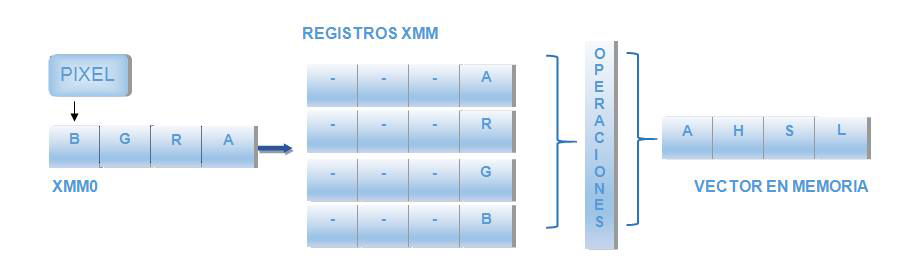
\includegraphics[width=130mm]{imagenes/hsl/hsl2-1.png}
\caption{Desarrollo de HSL-ASM2.}
\end{figure}

Para realizar la conversión del formato HSL al formato rgb, necesitamos obtener algunos valores utilizando las fórmulas provistas por la cátedra, C, X y M, que los guardaremos en las partes bajas de XMM4, XMM5 y XMM6 respectivamente. Para calcular fabs utilizamos una mascara que pone en 0 el bit de signo, mientras que para calcular fmod utilizamos divisiones y conversiones a enteros y nuevamente a float para eliminar los decimales y poder hacer el calculo como muestra la figura. Luego procedemos a calcular los valores en formato rgb según los resultados de las funciones condicionales otorgadas también por la cátedra, utilizando la misma lógica sobre las condiciones como se hizo anteriormente en la función para transformar de rgb a HSL. En cada if, utilizamos instrucciones de SHUFFLE para ir modificando en caso de que sea necesario, los valores de R, G y B. El resultado de ésto es guardado en XMM4 y luego hacemos los cálculos de escala (multiplicar todas las componentes por 255) y los convertimos a enteros.

\begin{figure}[ht!]
\centering
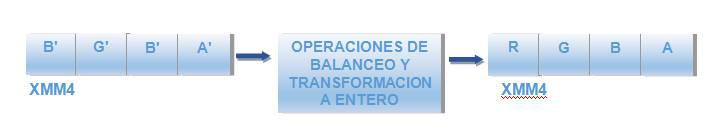
\includegraphics[width=100mm]{imagenes/hsl/hsl2-2.png}
\caption{Desarrollo de HSL-ASM2.}
\end{figure}

Para finalizar, volvemos las componentes a su tamaño original en la parte baja de XMM4 y lo guardamos en su posición original en la imagen.

\begin{figure}[ht!]
\centering
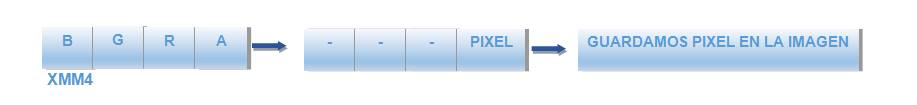
\includegraphics[width=130mm]{imagenes/hsl/hsl2-3.png}
\caption{Desarrollo de HSL-ASM2.}
\end{figure}
